\documentclass[11pt,a4paper]{article}
\usepackage[utf8]{inputenc}
\usepackage[T1]{fontenc}
\usepackage{lmodern}
\usepackage[margin=25mm]{geometry}
\usepackage{amsmath,amssymb,amsfonts,graphicx,booktabs,array,microtype}
\usepackage[hidelinks]{hyperref}
\usepackage{orcidlink}
\graphicspath{{../figures/}}
\setlength{\parindent}{0pt}
\setlength{\parskip}{5pt}
\newcommand{\doctype}{Preprint}
\newcommand{\docversion}{v2.6 draft}
\newcommand{\docdate}{5 November 2026}
\newcommand{\versiondoi}{10.5281/zenodo.23884367}
\newcommand{\conceptdoi}{10.5281/zenodo.21508920}
\newcommand{\docrepo}{github.com/fsantibanezleal/CAOS\_RES\_ChronoScope}
\newcommand{\headerblock}{%
\begin{center}
\fbox{\parbox{0.94\textwidth}{\small\raggedright
\textbf{\doctype} \quad$\cdot$\quad \docversion, \docdate \quad$\cdot$\quad Licence CC BY 4.0\\[2pt]
CAOS open-research programme \quad$\cdot$\quad CAOS\_RES\_ChronoScope, time-series forecasting method atlas\\[2pt]
Published predecessor DOI: \versiondoi \quad$\cdot$\quad
concept DOI (always latest) \href{https://doi.org/\conceptdoi}{\texttt{\conceptdoi}}\\[2pt]
Not peer reviewed. Source code, data and computational records: \href{https://\docrepo}{\texttt{\docrepo}}
}}
\end{center}}

\hypersetup{pdftitle={Prequential Evaluation of Adaptive Prediction Intervals: A Fifteen-Series Replay Study},pdfauthor={Felipe Santibáñez-Leal}}
\begin{document}
\title{Prequential Evaluation of Adaptive Prediction Intervals: A Fifteen-Series Replay Study}
\author{Felipe Santib\'a\~nez-Leal~\orcidlink{0000-0002-0150-3246}\\CAOS open-research programme, Santiago, Chile\\\small \texttt{fsantibanezleal@ug.uchile.cl}}
\date{}
\maketitle
\begin{center}\textbf{Working revision; not a new published version.}\end{center}
\headerblock
\begin{abstract}

Adaptive prediction intervals can have accurate average coverage while retaining substantial local coverage error. We examine this distinction in a one-step prequential study of fifteen selected time series: eleven generated mechanisms and four real excerpts. The point forecaster is a full-history smoothing-plus-drift adaptation, rather than a native stateful forecaster or the standard finite-history Theta method. Two scale-normalized score-buffer controllers use ACI-style and PID-style updates of an effective miscoverage level. At nominal 80\% coverage, their mean rolling absolute coverage errors are 0.0656 and 0.0645, compared with 0.0830 for unadjusted intervals. The substantially smaller errors obtained by first averaging signed coverage deviations over time describe a different statistic and do not establish uniformly accurate local coverage. Every numerical forecast, target, score and controller update is reconstructed and checked against the archived coverage trajectories and final weighted quantile losses. Sensitivity calculations vary nominal coverage, base forecaster, controller gains and generated-series seeds. These selected finite-stream results characterize the evaluated implementations; they provide neither a new coverage theorem nor a general forecasting advantage.
\end{abstract}

\section{Question and relation to prior work}
A sequential interval forecast must use information available before its target arrives. Its quality has at least two dimensions: coverage and concentration. An interval can obtain high coverage by becoming excessively wide; a long-run coverage average can also conceal sustained local deviations. We ask how two particular adaptive interval controllers behave on a selected collection when these distinctions are made explicit.

Prequential evaluation scores predictions before incorporating their outcomes~\cite{dawid1984}. Adaptive Conformal Inference (ACI) adapts an effective miscoverage level~\cite{gibbs2021}. Conformal PID Control combines control-theoretic ideas with prospective conformal score forecasting~\cite{angelopoulos2023}. The evaluated algorithms build on these precedents. The PID-style controller evaluated here acts on a bounded effective miscoverage level and uses an empirical score buffer. It is not a faithful implementation or comparative evaluation of the published Conformal PID algorithm, and that algorithm's guarantees are not assigned to it.

The contribution is a reproducible, implementation-specific comparison of global and local empirical coverage measures, interval efficiency, and sensitivity on the same streams. The software package \texttt{preqts} supplies the replay interface and archived controllers. The experiment compares interval rules; it does not compare native model-state updates or establish a capability gap in other evaluation frameworks.

\section{Data and sequential information}
The collection contains fifteen deliberately selected cases: eleven generated mechanisms and four real excerpts. Generated mechanisms include daily seasonality, trend with seasonality, intermittent demand, a near-random walk, white noise, level changes, multiple seasonalities, heteroskedasticity, long memory, nonlinear Mackey--Glass dynamics and a promotion covariate example. Real excerpts comprise UCI electricity, Beijing PM2.5, M4 hourly and M4 daily. They do not constitute random draws from a forecasting population. White noise and the near-random walk are negative controls, not proofs that every form of leakage is absent.

Let $y_0,\ldots,y_{T-1}$ be the complete stream and $m$ its configured seasonal lag. The initial prefix has length
\begin{equation}
w=\min\{\max(2m,20),\max(1,\lfloor T/3\rfloor)\}.
\end{equation}
At $t=w,\ldots,T-1$, every method predicts $y_t$ using $y_{0:t-1}$. The target is then revealed, the forecast is scored, and the prefix and controller are updated. Horizon and advance are both one. This streaming experiment includes the full case sequence; its targets must not be pooled with the separate final-block experiment in the surrounding atlas.

\begin{figure}[htbp]\centering
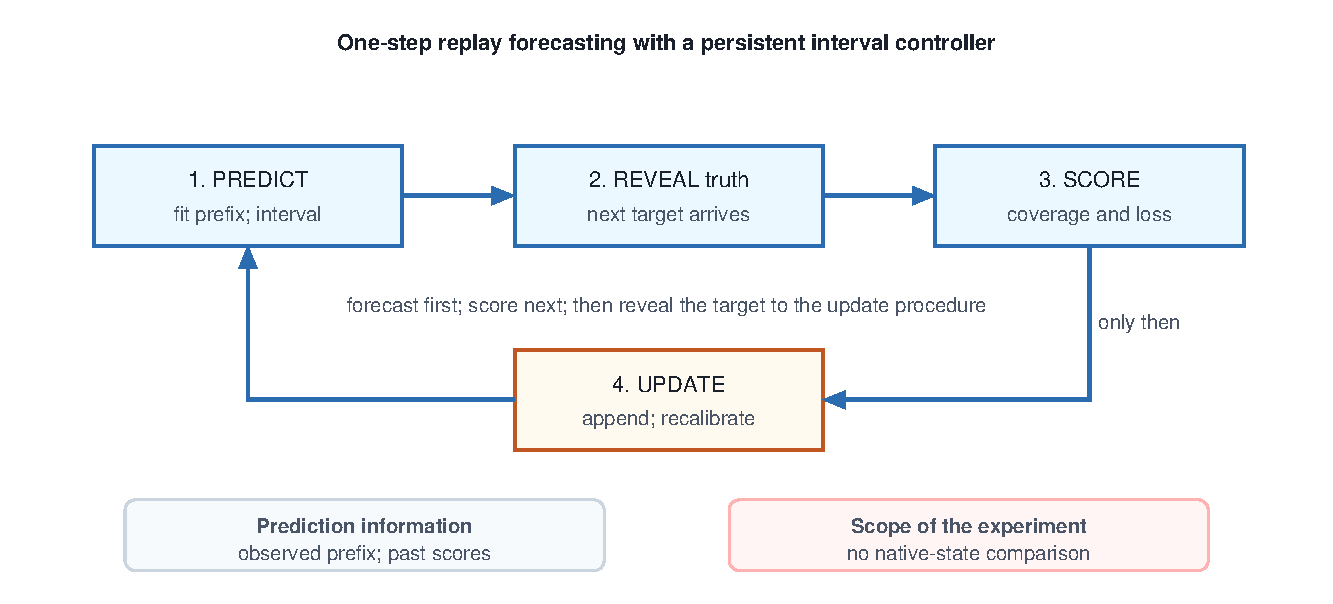
\includegraphics[width=.86\textwidth]{fig-prequential.pdf}
\caption{Information order in the evaluated replay implementation. The point method is recomputed on the observed prefix; an interval controller carries its own scores and level between arrivals. The next target enters either update only after scoring. This diagram makes no comparison with other forecasting frameworks or native state-update costs.}
\label{fig:prequential}\end{figure}

The numerical reconstruction retains the full-precision source values, generator definitions and seeds, case identities, seasonal lags and initial-prefix lengths. SHA-256 values bind each source array, admitted real-data CSV, generator implementation, case manifest, display trace and archived streaming artifact. Every displayed sample and reserved final-block target is matched to the original indexed source within its four-decimal export tolerance. These bindings identify the actual experimental inputs, even where a historical upstream download revision or timing environment is unavailable. Covariates are not supplied to the four interval methods, including for the promotion case; no covariate-availability result is inferred here.

\section{Point forecasts and base intervals}
We call the archived adaptation smoothing plus drift (S+D). The historical artifact key \texttt{Theta} identifies this implementation, but it lacks the finite-history correction of the standard nonseasonal Theta representation~\cite{hyndman2003}. For the observed prefix $x_0,\ldots,x_{n-1}$, an OLS line against integer time gives slope $b$. A smoothing coefficient $a$ is selected from $\{.05,.10,\ldots,.95\}$ by minimum in-sample one-step squared error. With $\ell_0=x_0$,
\begin{equation}
\ell_i=a x_i+(1-a)\ell_{i-1},\qquad
p_t=\ell_{n-1}+\tfrac12 b.
\end{equation}
The fitted value for $x_i$ is $\ell_{i-1}$; $\hat\sigma_t$ is the population standard deviation of these residuals for $i=1,\ldots,n-1$. At nominal coverage $c$, the base half-width is $\Phi^{-1}((1+c)/2)\hat\sigma_t$, using the package's Acklam normal-quantile approximation. This Gaussian approximation has no distribution-free coverage guarantee.

A second base is seasonal naive, $p_t=y_{t-m}$, with dispersion equal to the population standard deviation of observed lag-$m$ differences. The historical comparison contains seasonal naive and raw S+D, plus two calibrated versions of S+D. The sensitivity comparison applies the same controllers to both bases. Both are full-prefix replay calculations; the point forecasts do not become streaming-native merely because the interval controller has persistent state.

\section{Adaptive interval rules}
For a base median $p_t$ and half-width $r_t=\max(\Phi^{-1}((1+c)/2)\hat\sigma_t,10^{-8})$, a FIFO buffer retains at most 200 past scores
\begin{equation}
z_j=|y_j-p_j|/r_j,\qquad j<t.
\end{equation}
Before forecasting $y_t$, $q_t$ is the buffered sample quantile at level $1-\alpha_t$, using NumPy's default linear interpolation. An empty buffer gives $q_t=1$. Endpoints are $p_t\pm q_t r_t$. Only after scoring is $z_t$ appended. This is a normalized-residual buffer rule, not a finite-sample split-conformal construction.

Let $e_t=\mathbf1\{z_t>q_t\}$, $\alpha^*=1-c$, and initialize $\alpha_w=\alpha^*$. The ACI-style update is
\begin{equation}
\alpha_{t+1}=\operatorname{clip}(\alpha_t+\gamma(\alpha^*-e_t),10^{-4},1-10^{-4}),
\end{equation}
with $\gamma=.02$. Level clipping and the interpolated finite score buffer are part of this evaluated variant; the ACI paper's theoretical guarantee is not claimed for it without further argument.

For the PID-style rule, set $u_t=\alpha^*-e_t$, $I_t=I_{t-1}+u_t$ with initial integral zero, and $d_t=u_t-u_{t-1}$, using zero derivative on the first update. Then
\begin{equation}
\alpha_{t+1}=\operatorname{clip}(\alpha^*+k_pu_t+k_iI_t+k_dd_t,10^{-4},1-10^{-4}),
\end{equation}
where $(k_p,k_i,k_d)=(.05,.02,.02)$. The integral is not separately clipped. Unlike the ACI recursion, this rule recomputes the level around $\alpha^*$ from all three terms. The median is unchanged by either controller.

The gains are inherited fixed software settings. No historical parameter-selection rationale, optimality study or independent tuning set is available. Sensitivity uses all multipliers $g\in\{.5,1,2\}$, multiplying $\gamma$ or all three PID gains together. It does not choose and re-evaluate the best multiplier. Nominal coverages are $.7,.8,.9$. The full design gives $15\times2\times3\times(1+3+3)=630$ case-setting rows, including raw references.

\section{Metrics and numerical reconstruction}
For case $i$, write $B_{it}=\mathbf1\{l_{it}\le y_{it}\le u_{it}\}$ and let $C_{it}$ be its trailing coverage mean over at most 25 cutoffs, including $t$. With $N=15$ cases and $K_i$ cutoffs, three different errors are
\begin{align}
E_{\rm avg}&=N^{-1}\sum_i\left|K_i^{-1}\sum_t C_{it}-c\right|,\\
E_{\rm roll}&=N^{-1}\sum_i K_i^{-1}\sum_t|C_{it}-c|,\\
E_{\rm final}&=N^{-1}\sum_i\left|K_i^{-1}\sum_t B_{it}-c\right|.
\end{align}
$E_{\rm avg}$ permits temporal cancellation within each case; $E_{\rm roll}$ does not. Neither is a conditional-coverage guarantee, and overlapping rolling windows are not independent observations. Archived $C_{it}$ values are rounded to five decimals; the reproduction uses that same rounding for these comparisons. Equal case weights prevent longer streams from dominating the summary.

Width is $u_t-l_t$. The central interval score is
\begin{equation}
\operatorname{IS}_t=(u_t-l_t)+\frac{2}{1-c}\{(l_t-y_t)_+ +(y_t-u_t)_+\},
\end{equation}
where only the violated side contributes~\cite{gneiting2007}. For cross-case summaries, width and interval score are divided by the mean absolute lag-$m$ difference in that case's initial prefix. This is the same fixed information set used for scaling one-step absolute error; final targets do not determine the scale.

At levels $q\in\{.1,.5,.9\}$, the archived WQL is $2\sum_q\rho_q(y_t-Q_{tq})/|y_t|$, where $\rho_q(v)=v(q-\mathbf1\{v<0\})$. It is unavailable when $y_t=0$. This per-cutoff ratio is not a pooled all-time denominator or a CRPS estimate. Its archive comparison averages available cutoff values. We do not optimize or headline this ratio, whose denominator can be unstable near zero.

The reconstruction exports 21,296 method-cutoff rows, each containing the target, three forecast columns, normalized score, multiplier, effective level before and after update, integral, derivative and buffer size. Previous score rows determine the entire FIFO contents. All fifteen archived coverage trajectories and final WQL summaries agree at their saved precision. Unit checks compare controller forecasts and levels directly with \texttt{preqts==0.3.0} and verify that changing a future target cannot alter an earlier forecast. A separate clean-process recomputation checks the complete numerical payload. The reconstruction is not an independent statistical replication, and it does not recover historical hardware or per-call latency.

\section{Results}
\begin{table}[htbp]\centering\footnotesize
\caption{Coverage errors on the same fifteen cases at nominal 80\%. The three columns are distinct statistics defined in the text; none is a confidence interval.}
\label{tab:coverage}
\begin{tabular}{lrrr}
\toprule
Method & $E_{\rm avg}$ & $E_{\rm roll}$ & $E_{\rm final}$\\\midrule
Seasonal naive & 0.0599 & 0.1309 & 0.0620\\
S+D & 0.0416 & 0.0830 & 0.0444\\
S+D + ACI-style & 0.0057 & 0.0656 & 0.0075\\
S+D + PID-style & 0.0060 & 0.0645 & 0.0074\\
\bottomrule\end{tabular}\end{table}

\begin{table}[htbp]\centering\footnotesize
\caption{Interval width and interval score divided by each case's warmup seasonal-difference scale, then averaged equally over cases. Lower interval score is better; smaller width alone is not.}
\label{tab:efficiency}
\begin{tabular}{lrr}
\toprule
Method & Scaled width & Scaled score\\\midrule
Seasonal naive & 4.2454 & 6.7012\\
S+D & 2.8403 & 4.0886\\
S+D + ACI-style & 2.7574 & 4.0808\\
S+D + PID-style & 2.7855 & 4.0834\\
\bottomrule\end{tabular}\end{table}

At nominal 80\%, raw S+D has $E_{\rm roll}=.0830$, compared with $.0656$ for the ACI-style rule and $.0645$ for the PID-style rule. This is a descriptive reduction of roughly 21\% and 22\% on these cases. By contrast, $E_{\rm avg}$ falls from $.0416$ to $.0057$ and $.0060$. The sevenfold ratio for the latter statistic does not describe local rolling error. Reporting these quantities under a single heading of calibration error would conceal their different interpretations.

\begin{figure}[htbp]\centering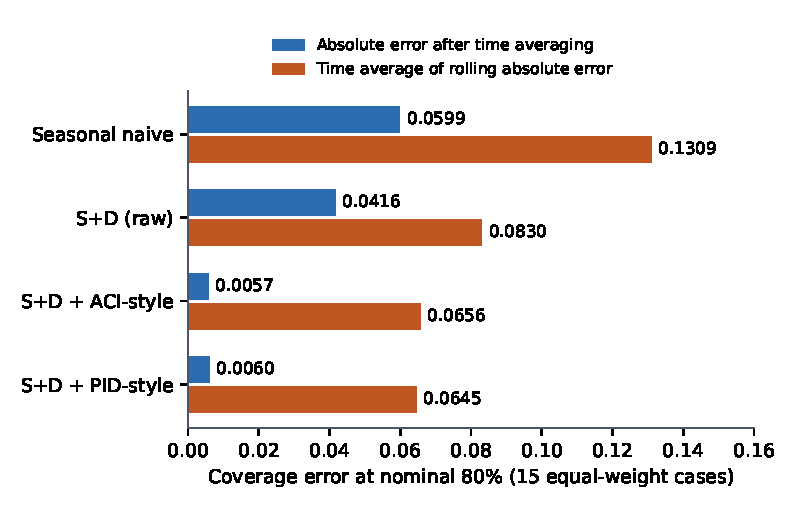
\includegraphics[width=.8\linewidth]{fig-coverage-summary.pdf}
\caption{Two coverage-error summaries on the same fifteen streams. Time-averaging before taking absolute deviations permits cancellation; averaging rolling absolute deviations measures a different property. Both remain descriptive finite-stream measurements.}\label{fig:summary}\end{figure}
\begin{figure}[htbp]\centering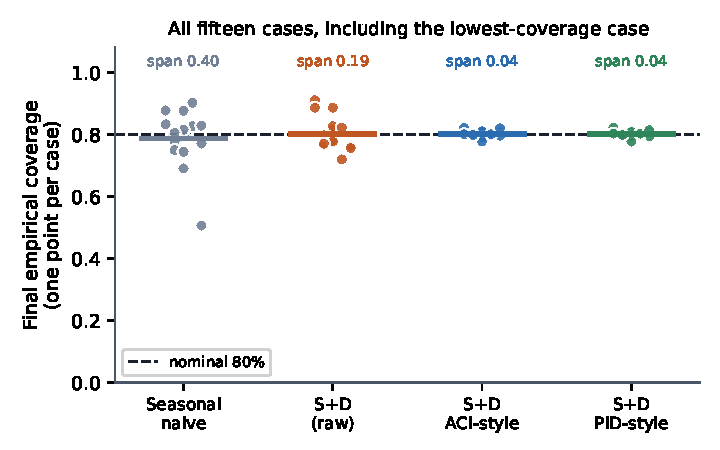
\includegraphics[width=.8\linewidth]{fig-coverage-percase.pdf}
\caption{Final empirical coverage at nominal 80\%, one point per case. The spread across cases is not a confidence interval or evidence of conditional coverage at each time.}\label{fig:percase}\end{figure}

The median forecast is identical across the three S+D interval rules by construction. Thus changes in interval quality do not demonstrate improved point forecasting. Scaled interval widths and scores quantify the accompanying concentration tradeoff, rather than treating coverage alone as sufficient.

\begin{table}[htbp]\centering\footnotesize
\caption{Mean rolling absolute error across fifteen cases. Controller cells give the range of the three fixed gain multipliers (0.5, 1, 2), not sampling uncertainty or a selected optimum.}
\begin{tabular}{lrrrr}
\toprule
Base & $c$ & Raw & ACI-style & PID-style\\\midrule
Seasonal naive & 0.7 & 0.1543 & 0.0976--0.1211 & 0.0907--0.1176\\
Seasonal naive & 0.8 & 0.1309 & 0.0849--0.1033 & 0.0774--0.1016\\
Seasonal naive & 0.9 & 0.0957 & 0.0629--0.0766 & 0.0596--0.0731\\
S+D & 0.7 & 0.1085 & 0.0712--0.0864 & 0.0667--0.0852\\
S+D & 0.8 & 0.0830 & 0.0597--0.0697 & 0.0558--0.0667\\
S+D & 0.9 & 0.0567 & 0.0499--0.0571 & 0.0494--0.0557\\
\bottomrule\end{tabular}\end{table}

\begin{table}[htbp]\centering\footnotesize
\caption{S+D base at nominal 80\%, default gains: mean rolling absolute error on eleven generated mechanisms for each seed. Seeds share generator definitions; real series are excluded from this table.}
\begin{tabular}{lrrr}
\toprule
Seed & Raw & ACI-style & PID-style\\\midrule
42 & 0.0684 & 0.0541 & 0.0525\\
43 & 0.0689 & 0.0580 & 0.0555\\
44 & 0.0693 & 0.0609 & 0.0587\\
\bottomrule\end{tabular}\end{table}

Sensitivity retains all 630 case-setting rows. At nominal 90\% on the S+D base, one ACI-style gain setting has slightly higher rolling absolute error than the raw interval, so improvement is not uniform across settings. A further calculation regenerates each of the eleven synthetic mechanisms at seeds 43 and 44, keeping its definition and controller settings fixed. Together with the original seed 42, these give three realizations per generated mechanism, not 33 independent real-world datasets. The four real excerpts have no artificial repeated seed and are not counted in the generated-only table. These analyses assess numerical sensitivity of the specified design; they are not prospective validation on an independently selected collection.

\section{Limitations and interpretation}
The study has one-step forecasts, short selected streams, two lightweight base constructions, three nominal levels and three gain multipliers. The bases share Gaussian dispersion approximations. There is no native stateful forecasting comparison, faithful published Conformal PID comparator, population sampling design, dependence-aware significance claim or operational cost study. A parameter range explored on these same cases cannot establish robustness outside it.

The numerical reproduction closes the missing per-update forecast and controller-state gap for the reconstructed experiment. It cannot retroactively supply a rationale for the original gains, the original machine's environment, or unavailable upstream acquisition revisions. Input hashes identify the exact redistributed values; they do not establish that those values represent all source-dataset populations. Historical measured latencies are therefore excluded from numerical-performance conclusions.

Improved empirical coverage in this construction is compatible with substantial local error, wider intervals or other unmeasured failure modes. The selected negative controls and information-order tests support bounded checks; they do not prove freedom from every possible leak. The appropriate conclusion is lower measured rolling coverage error for these particular controllers and streams, with interval efficiency and sensitivity reported alongside it.

\section*{Data and code availability}
The source, full numerical replay, sensitivity rows, input hashes and deterministic figure/table generators are at \url{https://github.com/fsantibanezleal/CAOS_RES_ChronoScope}. In a declared product environment, use Python to run \path{scripts/manuscript_replay.py} with \texttt{--check}, then run \path{scripts/make_manuscript_tables.py}. The streaming manuscript directory contains the numerical replay as \path{evidence/replay.json}. Source values are included for each case; raw upstream acquisition histories and original timing metadata are not reconstructed. The separately published \texttt{preqts==0.3.0} package supplies the checked historical controller implementation. Code and redistributed data retain their stated licences; prose uses the licence in the header.

\begin{thebibliography}{9}
\bibitem{dawid1984} A. P. Dawid, ``Statistical theory: The prequential approach,'' \emph{JRSS A}, vol. 147, no. 2, pp. 278--292, 1984, doi:10.2307/2981683.
\bibitem{gibbs2021} I. Gibbs and E. Cand\`es, ``Adaptive conformal inference under distribution shift,'' \emph{NeurIPS}, 2021, \url{https://arxiv.org/abs/2106.00170}.
\bibitem{angelopoulos2023} A. N. Angelopoulos, E. Cand\`es and R. J. Tibshirani, ``Conformal PID control for time series prediction,'' \emph{NeurIPS}, 2023, \url{https://arxiv.org/abs/2307.16895}.
\bibitem{hyndman2003} R. J. Hyndman and B. Billah, ``Unmasking the Theta method,'' \emph{International Journal of Forecasting}, vol. 19, no. 2, pp. 287--290, 2003, \url{https://robjhyndman.com/papers/Theta.pdf}.
\bibitem{gneiting2007} T. Gneiting and A. E. Raftery, ``Strictly proper scoring rules, prediction, and estimation,'' \emph{JASA}, vol. 102, no. 477, pp. 359--378, 2007, doi:10.1198/016214506000001437.
\end{thebibliography}
\end{document}
